\documentclass[border=10pt]{standalone}
\usepackage{tikz}
\usepackage{amsmath}
\usetikzlibrary{arrows.meta,positioning,matrix}

\definecolor{inFill}{RGB}{183,224,177}
\definecolor{inLine}{RGB}{32,102,32}
\definecolor{hidFill}{RGB}{199,203,243}
\definecolor{hidLine}{RGB}{52,58,143}
\definecolor{outFill}{RGB}{243,199,199}
\definecolor{outLine}{RGB}{143,52,52}
\definecolor{biasFill}{RGB}{255,241,194}
\definecolor{biasLine}{RGB}{171,122,34}
\definecolor{opFill}{RGB}{250,250,250}
\definecolor{opLine}{RGB}{70,70,70}
\definecolor{lineC}{RGB}{38,44,110}

\begin{document}
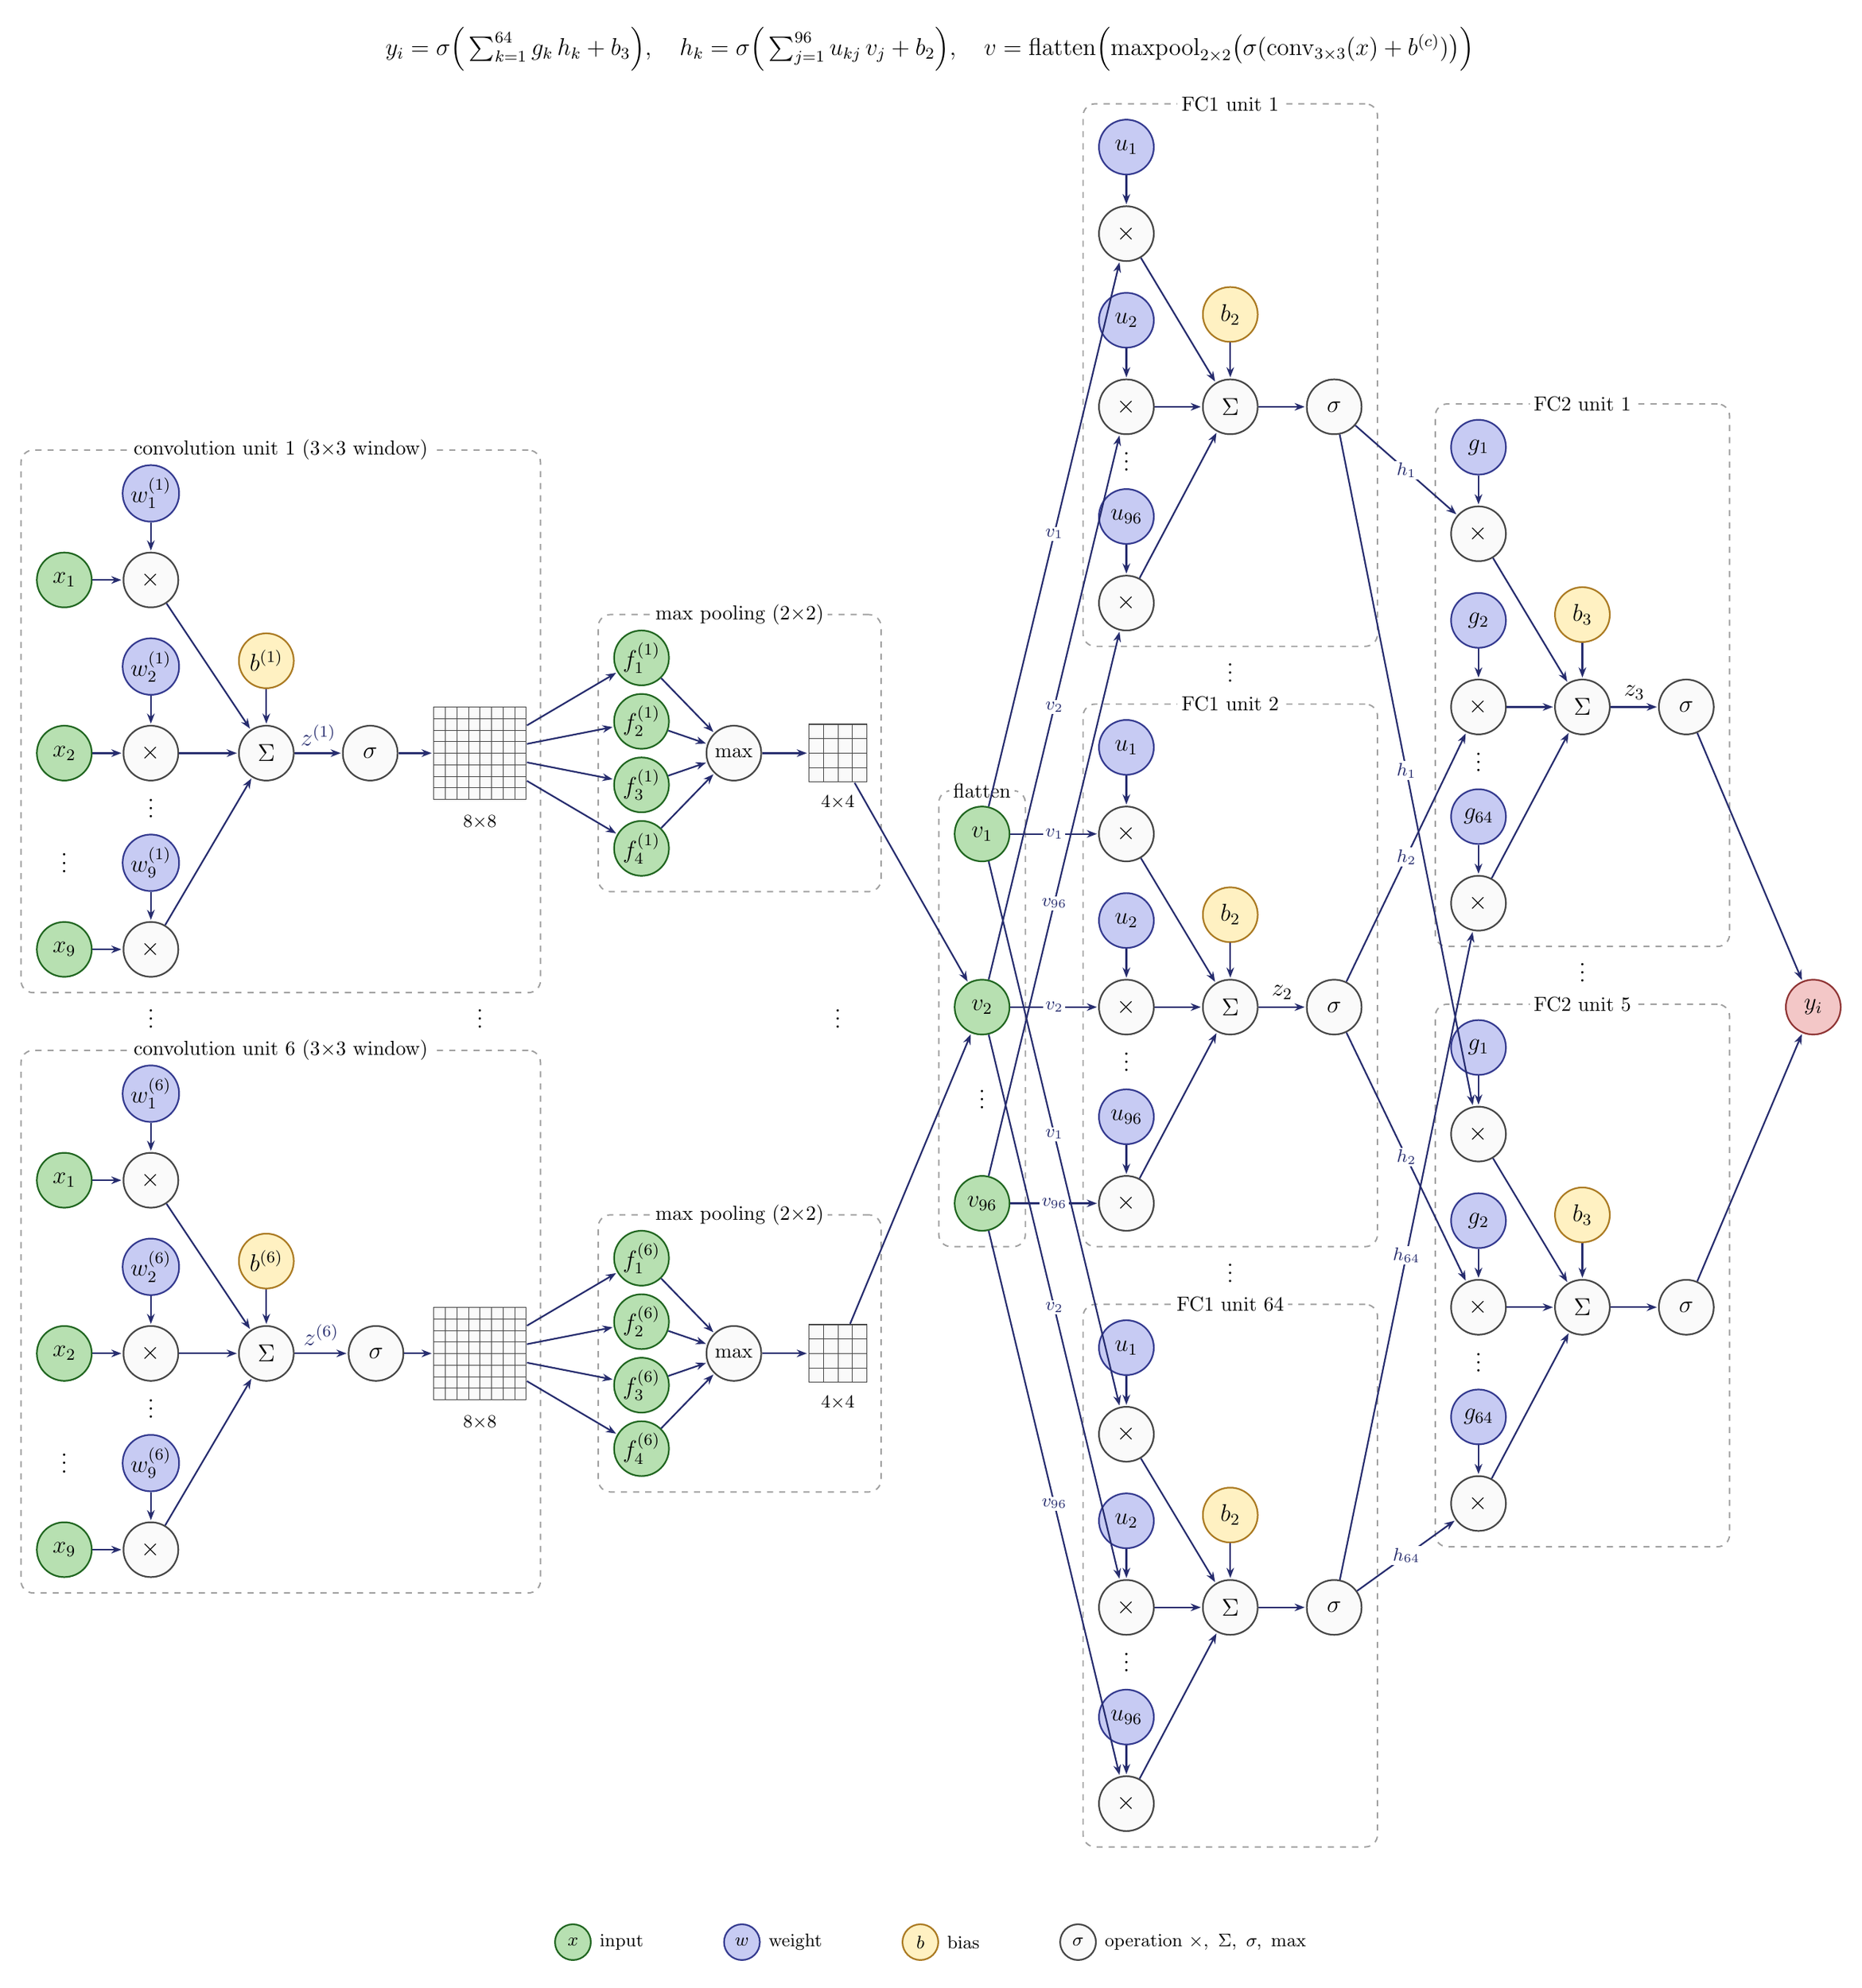
\begin{tikzpicture}[
    >={Stealth[length=5pt]}, line width=0.8pt, font=\large,
    op/.style  ={circle, draw=opLine, fill=opFill, minimum size=0.95cm, inner sep=0pt},
    leaf/.style={circle, minimum size=0.95cm, inner sep=1pt},
    inp/.style ={leaf, draw=inLine, fill=inFill},
    outp/.style={leaf, draw=outLine, fill=outFill},
    wgt/.style ={leaf, draw=hidLine, fill=hidFill},
    bia/.style ={leaf, draw=biasLine, fill=biasFill},
    dots/.style={circle, minimum size=0.95cm, inner sep=0pt},
    arr/.style ={lineC, ->, shorten >=0.6pt},
    nbox/.style={draw=gray!75, line width=0.7pt, dashed, rounded corners=6pt},
    elab/.style={midway, fill=white, inner sep=1pt, font=\small},
  ]

  % ---- 虚线框（★ 块间净空统一 1.0：pool +0.8, flatten +1.3, FC1 +0.8, FC2 不动）----
  \node[nbox, minimum width=9.0cm, minimum height=9.4cm] at (3.75, 4.95)  {};   % conv1（不动）
  \node[nbox, minimum width=4.9cm, minimum height=4.8cm] at (11.7, 4.4)   {};   % pool1
  \node[nbox, minimum width=1.5cm, minimum height=7.9cm] at (15.9,-0.2)   {};   % flatten / v 列
  \node[nbox, minimum width=9.0cm, minimum height=9.4cm] at (3.75,-5.45)  {};   % conv6（不动）
  \node[nbox, minimum width=4.9cm, minimum height=4.8cm] at (11.7,-6.0)   {};   % pool6
  \node[nbox, minimum width=5.1cm, minimum height=9.4cm] at (20.2,10.95)  {};   % FC1 unit 1
  \node[nbox, minimum width=5.1cm, minimum height=9.4cm] at (20.2, 0.55)  {};   % FC1 unit 2
  \node[nbox, minimum width=5.1cm, minimum height=9.4cm] at (20.2,-9.85)  {};   % FC1 unit 64
  \node[nbox, minimum width=5.1cm, minimum height=9.4cm] at (26.3, 5.75)  {};   % FC2 unit 1（回到原始位置）
  \node[nbox, minimum width=5.1cm, minimum height=9.4cm] at (26.3,-4.65)  {};   % FC2 unit 5
  \node[fill=white, inner sep=2pt, font=\normalfont] at (3.75, 9.65)  {convolution unit 1 (3$\times$3 window)};
  \node[fill=white, inner sep=2pt, font=\normalfont] at (11.7, 6.8)   {max pooling (2$\times$2)};
  \node[fill=white, inner sep=2pt, font=\normalfont] at (15.9, 3.75)  {flatten};
  \node[fill=white, inner sep=2pt, font=\normalfont] at (3.75,-0.75)  {convolution unit 6 (3$\times$3 window)};
  \node[fill=white, inner sep=2pt, font=\normalfont] at (11.7,-3.6)   {max pooling (2$\times$2)};
  \node[fill=white, inner sep=2pt, font=\normalfont] at (20.2,15.65)  {FC1 unit 1};
  \node[fill=white, inner sep=2pt, font=\normalfont] at (20.2, 5.25)  {FC1 unit 2};
  \node[fill=white, inner sep=2pt, font=\normalfont] at (20.2,-5.15)  {FC1 unit 64};
  \node[fill=white, inner sep=2pt, font=\normalfont] at (26.3,10.45)  {FC2 unit 1};
  \node[fill=white, inner sep=2pt, font=\normalfont] at (26.3, 0.05)  {FC2 unit 5};

  % ---- 整张图对应的复合函数（★ 水平居中 x=15.0）----
  \node[font=\large] at (15.0,16.6)
    {$y_i=\sigma\Big(\sum_{k=1}^{64} g_k\,h_k+b_3\Big),\quad
      h_k=\sigma\Big(\sum_{j=1}^{96} u_{kj}\,v_j+b_2\Big),\quad
      v=\mathrm{flatten}\Big(\mathrm{maxpool}_{2\times2}\big(\sigma(\mathrm{conv}_{3\times3}(x)+b^{(c)})\big)\Big)$};

  % ---- 第1行：卷积单元1（conv 组不动）----
  \node[inp] (r1x1) at (0,7.4) {$x_1$};
  \node[inp] (r1x2) at (0,4.4) {$x_2$};
  \node[dots] (r1xV) at (0,2.6) {$\vdots$};
  \node[inp] (r1x9) at (0,1.0) {$x_9$};
  \node[op] (r1m1) at (1.5,7.4) {$\times$};
  \node[op] (r1m2) at (1.5,4.4) {$\times$};
  \node[dots] (r1mV) at (1.5,3.55) {$\vdots$};
  \node[op] (r1m9) at (1.5,1.0) {$\times$};
  \node[wgt] (r1w1) at (1.5,8.9) {$w^{(1)}_1$};
  \node[wgt] (r1w2) at (1.5,5.9) {$w^{(1)}_2$};
  \node[wgt] (r1w9) at (1.5,2.5) {$w^{(1)}_9$};
  \node[op] (r1s) at (3.5,4.4) {$\Sigma$};
  \node[bia] (r1b) at (3.5,6.0) {$b^{(1)}$};
  \node[op] (r1a) at (5.3,4.4) {$\sigma$};
  \begin{scope}[shift={(7.2,4.4)}]
    \fill[opFill] (-0.8,-0.8) rectangle (0.8,0.8);
    \foreach \i in {1,...,7} \draw[opLine, line width=0.2pt] (-0.8+0.2*\i,-0.8) -- ++(0,1.6);
    \foreach \j in {1,...,7} \draw[opLine, line width=0.2pt] (-0.8,-0.8+0.2*\j) -- ++(1.6,0);
    \draw[opLine, line width=0.5pt] (-0.8,-0.8) rectangle (0.8,0.8);
  \end{scope}
  \node[inner sep=0pt, minimum size=1.6cm] (r1map) at (7.2,4.4) {};
  \node[font=\small] at (7.2,3.2) {8$\times$8};
  % pool 组 ★ +0.8
  \node[inp] (r1f1) at (10.0,6.05) {$f^{(1)}_1$};
  \node[inp] (r1f2) at (10.0,4.95) {$f^{(1)}_2$};
  \node[inp] (r1f3) at (10.0,3.85) {$f^{(1)}_3$};
  \node[inp] (r1f4) at (10.0,2.75) {$f^{(1)}_4$};
  \node[op, font=\normalsize] (r1mp) at (11.6,4.4) {max};
  \begin{scope}[shift={(13.4,4.4)}]
    \fill[opFill] (-0.5,-0.5) rectangle (0.5,0.5);
    \foreach \i in {1,...,3} \draw[opLine, line width=0.2pt] (-0.5+0.25*\i,-0.5) -- ++(0,1.0);
    \foreach \j in {1,...,3} \draw[opLine, line width=0.2pt] (-0.5,-0.5+0.25*\j) -- ++(1.0,0);
    \draw[opLine, line width=0.5pt] (-0.5,-0.5) rectangle (0.5,0.5);
  \end{scope}
  \node[inner sep=0pt, minimum size=1.0cm] (r1pmap) at (13.4,4.4) {};
  \node[font=\small] at (13.4,3.55) {4$\times$4};

  % ---- 第6行：卷积单元6（conv 组不动）----
  \node[inp] (r6x1) at (0,-3.0) {$x_1$};
  \node[inp] (r6x2) at (0,-6.0) {$x_2$};
  \node[dots] (r6xV) at (0,-7.8) {$\vdots$};
  \node[inp] (r6x9) at (0,-9.4) {$x_9$};
  \node[op] (r6m1) at (1.5,-3.0) {$\times$};
  \node[op] (r6m2) at (1.5,-6.0) {$\times$};
  \node[dots] (r6mV) at (1.5,-6.85) {$\vdots$};
  \node[op] (r6m9) at (1.5,-9.4) {$\times$};
  \node[wgt] (r6w1) at (1.5,-1.5) {$w^{(6)}_1$};
  \node[wgt] (r6w2) at (1.5,-4.5) {$w^{(6)}_2$};
  \node[wgt] (r6w9) at (1.5,-7.9) {$w^{(6)}_9$};
  \node[op] (r6s) at (3.5,-6.0) {$\Sigma$};
  \node[bia] (r6b) at (3.5,-4.4) {$b^{(6)}$};
  \node[op] (r6a) at (5.4,-6.0) {$\sigma$};
  \begin{scope}[shift={(7.2,-6.0)}]
    \fill[opFill] (-0.8,-0.8) rectangle (0.8,0.8);
    \foreach \i in {1,...,7} \draw[opLine, line width=0.2pt] (-0.8+0.2*\i,-0.8) -- ++(0,1.6);
    \foreach \j in {1,...,7} \draw[opLine, line width=0.2pt] (-0.8,-0.8+0.2*\j) -- ++(1.6,0);
    \draw[opLine, line width=0.5pt] (-0.8,-0.8) rectangle (0.8,0.8);
  \end{scope}
  \node[inner sep=0pt, minimum size=1.6cm] (r6map) at (7.2,-6.0) {};
  \node[font=\small] at (7.2,-7.2) {8$\times$8};
  % pool 组 ★ +0.8
  \node[inp] (r6f1) at (10.0,-4.35) {$f^{(6)}_1$};
  \node[inp] (r6f2) at (10.0,-5.45) {$f^{(6)}_2$};
  \node[inp] (r6f3) at (10.0,-6.55) {$f^{(6)}_3$};
  \node[inp] (r6f4) at (10.0,-7.65) {$f^{(6)}_4$};
  \node[op, font=\normalsize] (r6mp) at (11.6,-6.0) {max};
  \begin{scope}[shift={(13.4,-6.0)}]
    \fill[opFill] (-0.5,-0.5) rectangle (0.5,0.5);
    \foreach \i in {1,...,3} \draw[opLine, line width=0.2pt] (-0.5+0.25*\i,-0.5) -- ++(0,1.0);
    \foreach \j in {1,...,3} \draw[opLine, line width=0.2pt] (-0.5,-0.5+0.25*\j) -- ++(1.0,0);
    \draw[opLine, line width=0.5pt] (-0.5,-0.5) rectangle (0.5,0.5);
  \end{scope}
  \node[inner sep=0pt, minimum size=1.0cm] (r6pmap) at (13.4,-6.0) {};
  \node[font=\small] at (13.4,-6.85) {4$\times$4};

  % ---- 通道间省略号（D3 随 pool 组 +0.8）----
  \node[dots] (D1) at (1.5,-0.1)   {$\vdots$};
  \node[dots] (D2) at (7.2,-0.1)   {$\vdots$};
  \node[dots] (D3) at (13.4,-0.1)  {$\vdots$};

  % ---- flatten 框内的 v 列（★ +1.3）----
  \node[inp] (v1)  at (15.9, 3.0) {$v_1$};
  \node[inp] (v2)  at (15.9, 0)   {$v_2$};
  \node[dots](vV)  at (15.9,-1.5) {$\vdots$};
  \node[inp] (v96) at (15.9,-3.4) {$v_{96}$};

  % ---- FC1：3 个单元（★ +0.8）----
  \foreach \c/\Y in {1/10.4, 2/0, 3/-10.4} {
    \node[op]  (n1-\c)  at (18.4,{\Y+3.0})    {$\times$};
    \node[op]  (n2-\c)  at (18.4,\Y)          {$\times$};
    \node[dots](nV-\c)  at (18.4,{\Y-0.85})   {$\vdots$};
    \node[op]  (n96-\c) at (18.4,{\Y-3.4})    {$\times$};
    \node[wgt] (u1-\c)  at (18.4,{\Y+4.5})    {$u_1$};
    \node[wgt] (u2-\c)  at (18.4,{\Y+1.5})    {$u_2$};
    \node[wgt] (u96-\c) at (18.4,{\Y-1.9})    {$u_{96}$};
    \node[op]  (s2-\c)  at (20.2,\Y)          {$\Sigma$};
    \node[bia] (b2-\c)  at (20.2,{\Y+1.6})    {$b_2$};
    \node[op]  (a2-\c)  at (22.0,\Y)          {$\sigma$};
  }
  \node[dots] (FV1) at (20.2, 5.9) {$\vdots$};
  \node[dots] (FV2) at (20.2,-4.5) {$\vdots$};

  % ---- FC2：2 个单元（★ 净空 1.0 时正好回到原始坐标，不动）----
  \foreach \c/\Y in {1/5.2, 2/-5.2} {
    \node[op]  (q1-\c)  at (24.5,{\Y+3.0})  {$\times$};
    \node[op]  (q2-\c)  at (24.5,\Y)        {$\times$};
    \node[dots](qV-\c)  at (24.5,{\Y-0.85}) {$\vdots$};
    \node[op]  (q64-\c) at (24.5,{\Y-3.4})  {$\times$};
    \node[wgt] (g1-\c)  at (24.5,{\Y+4.5})  {$g_1$};
    \node[wgt] (g2-\c)  at (24.5,{\Y+1.5})  {$g_2$};
    \node[wgt] (g64-\c) at (24.5,{\Y-1.9})  {$g_{64}$};
    \node[op]  (s3-\c)  at (26.3,\Y)        {$\Sigma$};
    \node[bia] (b3-\c)  at (26.3,{\Y+1.6})  {$b_3$};
    \node[op]  (a3-\c)  at (28.1,\Y)        {$\sigma$};
  }
  \node[dots] (HV1) at (26.3,0.7) {$\vdots$};

  % ---- 唯一输出 y（★ 30.3）----
  \node[outp] (y) at (30.3,0) {$y_i$};

  % ---- 边：卷积、池化 ----
  \draw[arr] (r1x1)--(r1m1); \draw[arr] (r1x2)--(r1m2); \draw[arr] (r1x9)--(r1m9);
  \draw[arr] (r1w1)--(r1m1); \draw[arr] (r1w2)--(r1m2); \draw[arr] (r1w9)--(r1m9);
  \draw[arr] (r1m1)--(r1s); \draw[arr] (r1m2)--(r1s); \draw[arr] (r1m9)--(r1s);
  \draw[arr] (r1b)--(r1s); \draw[arr] (r1s)--(r1a) node[midway, above] {$z^{(1)}$};
  \draw[arr] (r1a)--(r1map);
  \draw[arr] (r1map)--(r1f1); \draw[arr] (r1map)--(r1f2);
  \draw[arr] (r1map)--(r1f3); \draw[arr] (r1map)--(r1f4);
  \draw[arr] (r1f1)--(r1mp); \draw[arr] (r1f2)--(r1mp);
  \draw[arr] (r1f3)--(r1mp); \draw[arr] (r1f4)--(r1mp);
  \draw[arr] (r1mp)--(r1pmap);
  \draw[arr] (r6x1)--(r6m1); \draw[arr] (r6x2)--(r6m2); \draw[arr] (r6x9)--(r6m9);
  \draw[arr] (r6w1)--(r6m1); \draw[arr] (r6w2)--(r6m2); \draw[arr] (r6w9)--(r6m9);
  \draw[arr] (r6m1)--(r6s); \draw[arr] (r6m2)--(r6s); \draw[arr] (r6m9)--(r6s);
  \draw[arr] (r6b)--(r6s); \draw[arr] (r6s)--(r6a) node[midway, above] {$z^{(6)}$};
  \draw[arr] (r6a)--(r6map);
  \draw[arr] (r6map)--(r6f1); \draw[arr] (r6map)--(r6f2);
  \draw[arr] (r6map)--(r6f3); \draw[arr] (r6map)--(r6f4);
  \draw[arr] (r6f1)--(r6mp); \draw[arr] (r6f2)--(r6mp);
  \draw[arr] (r6f3)--(r6mp); \draw[arr] (r6f4)--(r6mp);
  \draw[arr] (r6mp)--(r6pmap);

  % ---- 池化 -> v 列 ----
  \draw[arr] (r1pmap)--(v2);
  \draw[arr] (r6pmap)--(v2);

  % ---- v -> 3 个 FC1 ----
  \foreach \c in {1,2,3} {
    \draw[arr] (v1)--(n1-\c)  node[elab] {$v_1$};
    \draw[arr] (v2)--(n2-\c)  node[elab] {$v_2$};
    \draw[arr] (v96)--(n96-\c) node[elab] {$v_{96}$};
  }

  % ---- FC1 内部 ----
  \foreach \c in {1,2,3} {
    \draw[arr] (n1-\c)--(s2-\c); \draw[arr] (n2-\c)--(s2-\c); \draw[arr] (n96-\c)--(s2-\c);
    \draw[arr] (u1-\c)--(n1-\c); \draw[arr] (u2-\c)--(n2-\c); \draw[arr] (u96-\c)--(n96-\c);
    \draw[arr] (b2-\c)--(s2-\c); \draw[arr] (s2-\c)--(a2-\c);
  }
  \path (s2-2)--(a2-2) node[midway, above] {$z_2$};

  % ---- 3 个 FC1 -> 2 个 FC2 ----
  \draw[arr] (a2-1)--(q1-1)  node[elab] {$h_1$};
  \draw[arr] (a2-1)--(q1-2)  node[elab] {$h_1$};
  \draw[arr] (a2-2)--(q2-1)  node[elab] {$h_2$};
  \draw[arr] (a2-2)--(q2-2)  node[elab] {$h_2$};
  \draw[arr] (a2-3)--(q64-1) node[elab] {$h_{64}$};
  \draw[arr] (a2-3)--(q64-2) node[elab] {$h_{64}$};

  % ---- FC2 内部 ----
  \foreach \c in {1,2} {
    \draw[arr] (g1-\c)--(q1-\c); \draw[arr] (g2-\c)--(q2-\c); \draw[arr] (g64-\c)--(q64-\c);
    \draw[arr] (q1-\c)--(s3-\c); \draw[arr] (q2-\c)--(s3-\c); \draw[arr] (q64-\c)--(s3-\c);
    \draw[arr] (b3-\c)--(s3-\c); \draw[arr] (s3-\c)--(a3-\c);
  }
  \path (s3-1)--(a3-1) node[midway, above] {$z_3$};

  % ---- FC2 -> 唯一输出 y ----
  \draw[arr] (a3-1)--(y);
  \draw[arr] (a3-2)--(y);

  % ---- 图例（★ 水平居中 x=15.0）----
  \matrix (leg) at (15.0,-16.2) [column sep=4pt, nodes={inner sep=0pt}] {
    \node[inp, minimum size=0.62cm, font=\small] {$x$}; &
    \node[font=\small] {input}; &
    \node[minimum width=1.1cm] {}; &
    \node[wgt, minimum size=0.62cm, font=\small] {$w$}; &
    \node[font=\small] {weight}; &
    \node[minimum width=1.1cm] {}; &
    \node[bia, minimum size=0.62cm, font=\small] {$b$}; &
    \node[font=\small] {bias}; &
    \node[minimum width=1.1cm] {}; &
    \node[op, minimum size=0.62cm, font=\small] {$\sigma$}; &
    \node[font=\small] {operation $\times,\ \Sigma,\ \sigma,\ \mathrm{max}$}; \\
  };
\end{tikzpicture}
\end{document}